\documentclass[a4paper,11pt]{article}

\usepackage[utf8]{inputenc}
\usepackage[T1]{fontenc}
\usepackage[english,french]{babel}
	\frenchbsetup{SmallCapsFigTabCaptions=false}
\usepackage{indentfirst}
\usepackage[margin=0.7in, bottom=0.7in, top=0.7in]{geometry}
\usepackage[table,kerneldraw,dvipsnames]{xcolor}
\usepackage{pdflscape}
\usepackage{rotating}

\usepackage{csquotes}
\usepackage[natbib=true,backend=biber,style=ieee,sort=none,sortcites=true,backref=true,backref=false
        language=french,autolang=other,url=true,isbn=true,doi=true]{biblatex}
\DefineBibliographyExtras{french}{\restorecommand\mkbibnamefamily}
\addbibresource{ref.bib}
\AtBeginBibliography{\small}

\usepackage{fancyhdr}
\pagestyle{fancy}
\fancyhead{}
\fancyhead[C]{\footnotesize \itshape A. Huat / Deep Learning (2018)}

\usepackage[nopostdot,nonumberlist,toc,acronyms]{glossaries}
\renewcommand{\glossarypreamble}{\small}

\usepackage{booktabs,array,longtable,tabularx}

\usepackage{menukeys}
\usepackage[shortcuts]{extdash}
\usepackage{enumitem}
%	\setlist{itemsep=0ex}
\usepackage{multicol}
\newenvironment{colfig}{\par\medskip\noindent\minipage{\linewidth}}{\endminipage\par\medskip}

\usepackage{float}
\usepackage{graphicx}
	% Centering figures by default
	\makeatletter
	\g@addto@macro\@floatboxreset{\centering}
	\makeatother
\usepackage{here}
\usepackage{placeins}
\usepackage[labelfont=bf,justification=justified]{caption}
    \captionsetup[table]{labelsep=newline,singlelinecheck=false,name={Tableau}}
    \captionsetup[figure]{labelsep=period}
%\usepackage{floatrow}
	\floatplacement{figure}{htbp}
	\floatplacement{table}{htbp}

\usepackage[colorlinks=true,plainpages=false,breaklinks=true,allcolors=NavyBlue]{hyperref}
\usepackage{fancyref}

\usepackage{listings,listingsutf8}
	\lstset{
		breaklines=true,
		deletekeywords={},
		frame=single,
		morekeywords={pour, chaque},
		tabsize=4,
		basicstyle=\scriptsize,
		escapeinside={lx*}{*lx}
}

% Maths

\usepackage{cool}
\usepackage{upgreek}
\usepackage{upref}
\usepackage{mathtools}
\usepackage{amsmath}
\usepackage{amsfonts}
\usepackage{amsthm}
\theoremstyle{definition}
\usepackage{amssymb}
\usepackage[scaled=1.]{rsfso}
\usepackage[scaled=1.,mathscr]{urwchancal}
\usepackage{stmaryrd}

% --------------------------------------
% Macros
% --------------------------------------

\newcommand{\fnhref}[2]{\href{#1}{#2}\footnote{#1}}

\newcommand{\TODO}[1]{\textsf{\color{orange}\bfseries TODO: #1}}

\newcommand{\ml}{\textit{machine learning}}
\newcommand{\ds}{\textit{data science}}

\newcommand{\cad}{c'est-à-dire}
\newcommand{\Cad}{C'est-à-dire}
\newcommand{\pex}{par exemple}
\newcommand{\Pex}{Par exemple}
\newcommand{\AH}{Alexandre Huat}
\newcommand{\eg}{\textit{e.g.}}
\newcommand{\ie}{\textit{i.e.}}
\newcommand{\etc}{\textit{etc.}}
\newcommand{\vs}{\textit{vs.}}
\newcommand{\cf}{\textit{cf.}}

% Maths

% --------------------------------------
% Glossaire
% --------------------------------------

\makeglossaries

%%% Acronyms

\newacronym[shortplural={qqc},longplural={qqc}]{qqc}{QQC}{quelque chose}

%%% Maths

% --------------------------------------
% Title
% --------------------------------------

\title{\Large\bfseries\textit{Differentially Private Releasing via Deep Generative Model} : Résumé}
\author{\textbf{\AH}\\{\small INSA Rouen Normandie\\Master Science des Données}}
\date{\today}

% ======================================

\begin{document}
\maketitle
\hrule height 1.6pt


% --------------------------------------
% Body
% --------------------------------------

\begin{multicols}{2}

Supposons des un groupe de clients et un prestateur de services informatiques collectant et analysant leurs données (\eg\ image, texte, audio). Afin de réaliser les tâches d'analyses, le prestateur est amené à traiter des données sensibles. Soucieux et/ou contraint de respecter la vie privée des clients, le prestateur doit trouver un moyen de traiter efficacement ces données tout en conservant leur confidentialité. Pour répondre à cette problématique, \citet{2018arXiv180101594Z} ont proposé l'architecture profonde dp-GAN\footnote{\textit{Differentially Private Generative Adversarial Network}}, que je résumerai ici. En particulier, dp-GAN offre (i) une garantie théorique à la préservation de la confidentialité des données via le principe de « confidentialité différentielle », \textcolor{(ii) retient  it retains desirable utility in the released model, enabling a variety of oth-erwise impossible analyses, et (iii) most importantly, it achieves practical training scalability and stability by employing multi-fold optimization strategies.}

dp-GAN est une architecture dont le rôle est de générer des données synthétiques mais sémantiquement riches qui pourront être utilisées sans violer la vie privée des utilisateurs, ou « clients » (\cf\ \autoref{dp-gan_role}).

\begin{colfig}
    \centering
    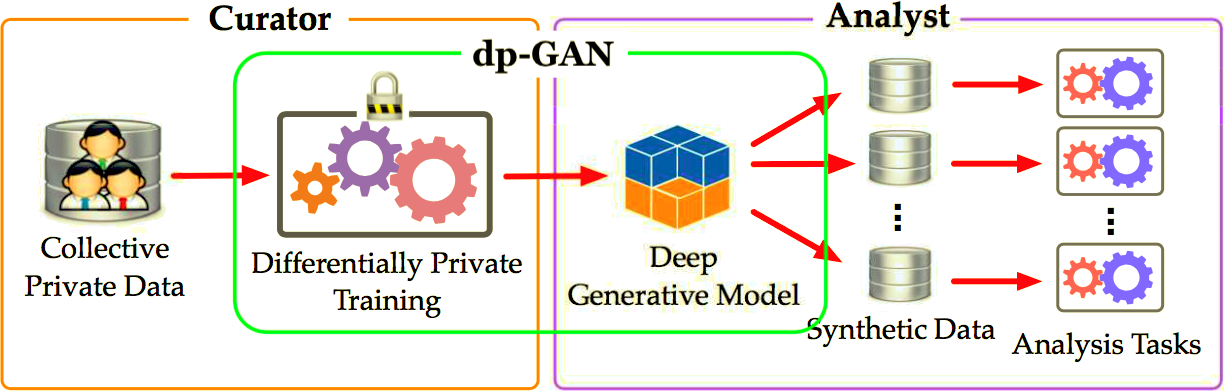
\includegraphics[width=\textwidth]{dp-gan_role.png}
    \captionof{figure}{La place de dp-GAN dans la chaîne de traitement des données privées}
    \label{dp-gan_role}
\end{colfig}

%\hrule
% \begin{otherlanguage}{english}
\printbibliography[title=Références] % ,heading=none
% \end{otherlanguage}

\end{multicols}
\end{document}
